%%%% Martin Rotter, Tomáš Kukučka - FJAA (zápisky z přednášek)
%%%%
%%%% kompilováno přes cslatex --> dvipdfmx

\documentclass[10pt, a4paper, titlepage]{article}

\usepackage{czech}						% napsáno česky
\usepackage[utf8]{inputenc}				% napsáno v UTF-8
\usepackage[tables,figures]{upreport}	% UPOL styl
\usepackage{upstyles}
\usepackage{a4wide}
\usepackage{amsmath}
\usepackage{amssymb}
\usepackage{amsthm}

\setlength{\parindent}{0pt}
\setlength{\parskip}{1ex plus 0.5ex minus 0.2ex}

\title{KMI/FJAA  -- Formální jazyky a automaty}
\author{M.~Rotter, T.~Kukučka}
\date{\today}

\docinfo{M.~Rotter, T.~Kukučka}{KMI/FJAA  -- Formální jazyky a automaty}

\newtheoremstyle{note}% name
{15pt}
{15pt}
{}
{}
{}
{:}
{.5em}
{}
\theoremstyle{note}
\newtheorem{veta}{\textbf{Věta}}
\newtheorem{definice}{\textbf{Definice}}
\newtheorem{dukaz}{\textbf{Důkaz}}
\newtheorem{priklad}{\textbf{Příklad}}
\newtheorem{dusledek}{\textbf{Důsledek}}

\abstract{Tento dokument je pouze přepisem zápisků a poznámek z přednášek předmětu KMI/FJAA. Přednášel \link{doc. Vilém Vychodil PhD}{http://vychodil.inf.upol.cz/}.}

\pagestyle{empty}
\makeindex

\begin{document}
\maketitle

\section{Historie}
Počátek úvah, jež byly později základem seriozního zkoumání formálních jazyků potažmo automatů se datuje do 30. let.
Průkopníkem této oblasti byl \link{Noam Chomsky}{http://cs.wikipedia.org/wiki/Noam_Chomsky}
\footnote{Jméno této osoby čti [\emph{čomski}] a zapamatuj si ke státnícím, že Chomski byl \emph{nebezpečný levicový intelektuál}.}.

Jako příklad selhání autora programovacího jazyka si uveďme jazyk \textbf{Fortran}, jehož konstrukce byla po syntaktické stránce špatná,
což vedlo ke \textbf{gramatické nejednoznačnosti} tohoto jazyka.

\section{Kódová analýza}
\subsection{Lexikální analýza}
Dělení kódu na tokeny\footnote{Překládej jako \emph{část, díl nebo také fráze}.}, jež se zapisují například ve stylu
$\langle\text{ znak, identifikátor }\rangle$.
Příkladem je tedy i token $\langle =, assignment \rangle$ a jiné.

\subsection{Syntaktická analýza}
Syntaktická analýza vytváři stromovou závislost jednotlivých tokenů, jejíž reprezentace se nazývá \textbf{syntaktický-derivační strom}.
V rámci této analýzy rozlišme:
\begin{enumerate}
\item
Teorii jazyků, jenž se zabýva stavbou jazyka (resp. jeho syntaxí) a poskytuje tzv. \emph{generativní aparát}.
Dodejme, že gramatika řiká, v jakém tvaru může být zapsán validní program.

\item
Teorii automatů, jež poskytuje tzv. \emph{analytický aparát}.
Dodejme, že automatem se rozumí de-facto jednoduchý algoritmus.
\end{enumerate}

\section{Základní pojmy}
\begin{itemize}
\item
\textbf{Symbol} (případně znak). Jedná se o syntaktický pojem (význam tedy nehraje roli), který představuje \emph{jméno} (analogicky k \emph{písmenu} z přirozeného jazyka).
Mezi symboly počítejme například \textbf{0, +, Š, while}.

\item
\textbf{Abeceda}. Abecedou rozumíme množinu (například množinu $X$) všech přípustných symbolů (znaků), přičemž taková množina je neprázdná (tedy $|x|>0$) a konečná.
Konečnost množiny je omezení dané reprezentovatelností množiny v rámci počitačové techniky.
Abecedy značíme řeckými písmeny. Například $\Sigma, \Sigma^{'}, \Gamma, \ldots, \Omega$.
Například $\Sigma = \lbrace a, b, c \rbrace$.

\item
\textbf{Řetězec} (případně slovo). Jedná se o konečnou posloupnost symbolů (znaků) vybraných z nějaké dané abecedy.
Například $\langle a_{1}, a_{2}, \ldots, a_{n} \rangle \in \Sigma, n$ nazvěme \emph{délkou řetězce}.
Formálně definujme řetězec jakožto \emph{zobrazení} $$x : \lbrace a, b, c, d, \ldots, i, j, \ldots \rbrace \rightarrow \Sigma $$
kde $$1 \rightarrow a, 2 \rightarrow b, 3 \rightarrow c$$ a tak podobně.
Délku řetězce označme $|x|$.

\item
\textbf{Prázdný řetězec}. Jedná se o řetěze, pro který platí, že $|x| = 0$ a značíme jej $\varepsilon$. Platí i následující zápis.
$$\varepsilon \subseteq \emptyset \rightarrow \Sigma$$
Prázdný řetězec \textbf{není} symbolem, tedy $\varepsilon \notin \Sigma$.
\end{itemize}

\begin{veta}
Nad $k$-prvkovou abecedou je právě $k^{n}$ řetězců délky $n$.
\end{veta}

\noindent
$\Sigma^{*}$ označuje množinu všech řetězců nad abecedou$\Sigma$. \\
$\Sigma^{+}$ označuje množinu všech řetězců nad abecedou$\Sigma$ vyjma $\varepsilon$.

\section{Operace s řetězci}
\begin{itemize}
\item
\textbf{Zřetězení} (konkatenace). Jde v podstatě o spojení\footnote{Pro milovníky jazyka Scheme můžeme tuto operaci přirovnat k proceduře \emph{append}}
dvou řetězců v daném pořadí do jednoho řetězce.

Mějme tyto řetezce. $$ a_{1}\ldots a_{n} \text{ a } b_{1}\ldots b_{m} $$
Pak jejich zřetězení má tvar $$ a_{1}\ldots a_{n}b_{1}\ldots b_{m} $$
Identifikátorem operace zřetězení je $\circ$, například $x\circ y$ je zřetězením řetězců $x$ a $y$.
Formálně takto.
\begin{gather*}
x : \lbrace 1,\ldots, n \rbrace \rightarrow \Sigma \\
y : \lbrace 1,\ldots, m \rbrace \rightarrow \Sigma \\
x \circ y : \lbrace 1,\ldots, nm \rbrace \rightarrow \Sigma
\end{gather*}

Algebraicky je \textbf{tatáž} operace zapsána jako $\langle \Sigma^{*}, \circ, \varepsilon \rangle$.

\item
\textbf{Rovnost řetězců}
Pro prohlášení dvou řetězců za sobě rovné v žádaném smyslu je třeba splnit obecně dvě podmínky.
\begin{enumerate}
\item
Oba řetězce mají stejnou délku, tedy $|x| = |y|$.

\item
Bude-li délka označena jako $n$, pak musí platit, že $\forall i | i \in \lbrace 1, \ldots, n \rbrace, x(i) = y(i)$.
Tedy každé dva k sobě náležící symboly z daných řetězců jsou si rovny.
\end{enumerate}
Uvažujeme-li rovnost řetězců, pak je záhodno uvažovat následující pojmy.
\begin{itemize}
\item
\textbf{Prefix} řetězce. Označme jej $Pfx(x) = \lbrace y | \exists z \text{ tak, že } yz = x \rbrace$.

\item
\textbf{Infix} řetězce. Označme jej $Ifx(x) = \lbrace y | \exists z_{1}, z_{2} \text{ tak, že } z_{1}yz_{2} = x \rbrace$.

\item
\textbf{Sufix} řetězce. Označme jej $Sfx(x) = \lbrace y | \exists z \text{ tak, že } zy = x \rbrace$.
\end{itemize}

\begin{veta}
\begin{gather*}
xy = xz \: \Longrightarrow \: y = z \\
yx = zx \: \Longrightarrow \: y = z
\end{gather*}
Algebraicky je operace zapsána jako $\langle \Sigma^{*}, \cdot, \varepsilon \rangle$.
\end{veta}

\begin{veta}
Vyslovme předpoklad, že platí $xy = uv$. Pak platí právě jedno z těchto tvrzení.
\begin{gather*}
x = u, y = v \\
|x| > |u| \text{ a } \exists w| w \neq \varepsilon, \text{ tak že } x = uw \text{ a } v = wy \\
|x| < |u| \text{ a } \exists w| w \neq \varepsilon, \text{ tak že } u = xw \text{ a } y = wv
\end{gather*}
\end{veta}

\item
\textbf{N-tá mocnina} řetězce.
$$ x^{n} = \left\lbrace
\begin{array}{l l}
x & \text{pro } n=1 \\
xx^{n-1} & \text{v ostatních případech} \\
\end{array}
\right\rbrace
$$
Respektive.
$$ x^{n} = \left\lbrace
\begin{array}{l l}
\varepsilon & \text{pro } n=0 \\
xx^{n-1} & \text{v ostatních případech} \\
\end{array}
\right\rbrace
$$
Mějte na paměti, že operace mocnění má vyšší prioritu než-li operace konkatenace (zřetězení).

\begin{veta}
Mějme $ u \text{ a } v \in \Sigma^{*}$, pak platí $uv = vu$ (komutativita), právě
tehdy, když $\exists z| z \in \Sigma^{*} \text{ a nezáporná celá čísla } p, q \text{ tak, že } u = z^{p} \text{ a } v=z^{a}$.
\end{veta}

Předpokládejme, že po $p, z, q$ máme $u = z^{p}, v = z^{q}$. Pak obecně platí následující zápis.
$$
uv = z^{p}z^{q} = z^{p+q} = z^{p} z^{q} = vu
$$

Předpokládejme, že $uv = vu$. Indukcí přes $|uv|$ předpokládáme, že tvrzení platí pro libovolné dva řetězce, jejichž délka zřetězení je menší
než-li $|uv|$. Mohou nastat tyto případy.
\begin{enumerate}
\item
$|u| = |v|, \text{ pak } u = v, \text{ pak } z = u, p = q = 1$

\item
$|u| < |v|$
\end{enumerate}

Berme v potaz také následující zápis doplněný obrázkem \ref{obr-1}

\begin{gather*}
uv = v \\
wu = v \\
uw = wu \\
|uw| < |uv|, \text{ tedy } \exists z, p, q  \text{ tak, že } u = z^{p}, w = z^{q}, v = z^{p+q}
\end{gather*}

\begin{figure}[ht]
\centering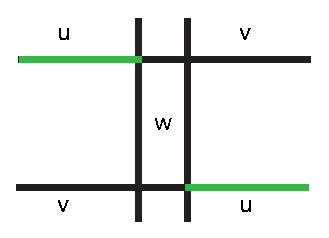
\includegraphics[width=5cm]{dukaz-1.eps}
\caption{Pomůcka k předchozímu tvrzení.}\label{obr-1}
\end{figure}
\end{itemize}

\section{Formální jazyk}
Definujme si pojem \emph{formální jazyk nad množinou (resp. abecedou)} $\Sigma^{*}$. Označme tento jazyk jako $L$. Pak platí tato tvrzení.
\begin{gather*}
L \subseteq \Sigma^{*} \text{ (každá podmnožina abecedy je jazykem)} \\
L = \emptyset \text{ (prázdný jazyk)} \\
L = \lbrace \varepsilon \rbrace \text{ (jazyk s prázdným řetězcem)} \\
L = jazyk C++ \text{ (jazyk C++)} \\
\vdots
\end{gather*}
\textbf{Pozor, obecně platí že prázdný jazyk $\neq$ jazyk s prázdným řetězcem.}
	
\section{Lexikografické uspořádání}
Předpokládejme uspořádání na množině $\Sigma^{*}$\footnote{Zopakujme si, že $\Sigma^{*}$ je množina všech řetězců nad $\Sigma$.}.
Nazvěme toto uspořádání \emph{striktním totálním}. Pak toto uspořádání například pro $\Sigma = \lbrace a_{1}, \ldots, a_{n} \rbrace$
je $a_{1} < a_{2} < a_{3} < \ldots < a_{n}$.

Totální striktní uspořádání označme $<_{l}$.

Položme $x <_{l} y$ pro $x,y \in \Sigma^{*}$. To ale platí pokud platí alespoň jedno z následujících dvou tvrzení.
\begin{enumerate}
\item
$|x| < |y|$

\item
$|x| < |y| \text{ a } \exists i \text{ tak, že } x(i) < y(i) \text{ a zároveň } x(j) < y(j) \text{ pro } \forall j |j < i$
\end{enumerate}

\begin{priklad}
$\Sigma = \lbrace 0, 1 \rbrace$. Triviálně tedy $0 < 1$.
Následně striktně $\varepsilon <_{l} 0 <_{l} 1 <_{l} 00 <_{l} 01 <_{l} 10 <_{l} 11$.
\end{priklad}

\begin{veta} \label{veta-1}
Striktní totální uspořádání je asymetrické a tranzitivní. A pro $x \neq y$ platí buď $x <_{l} y$ nebo $y <_{l} x$.
\INEM{problém}
\IN{problém!zapeklitý}
\IN{problém!zapeklitý!úplný}
\INEM{problém!a tady je ukázka dlouhého popisu}
\end{veta}

\begin{dusledek}
Důsledkem věty \ref{veta-1} je tvrzení, že množina $\Sigma^{*}$ je spočetně nekonečná. Dodejme, že jazyk je (obvykle) spočetná množina.
\end{dusledek}

\section{Operace nad jazyky}
\nextoutline{Mnozinové}
\subsection{Množinové}
Množinové operace nad jazyky jsou prakticky totožné operacím na kterýchkoliv jiných množinách. Můžeme tedy použít množinový průnik, sjednocení, komplement (doplněk) nebo rozdíl.
\subsection{Ostatní}
\begin{itemize}
\item
\textbf{Zřetězení} (produkt) množin. Vyjádřeme produkt takto.
$$L_{1}L_{2} = \lbrace xy | x \in L_{1}, y \in L_{2} \rbrace$$
Produkt množin není obecně komutativní, ale je asociativní, přičemž prázdná množina tuto operaci anihiluje.
Uveďme si rovněž monoid $\langle 2^{\Sigma^{*}}, \circ, \lbrace \varepsilon \rbrace \rangle$.
% Neneutrálním prvkem by byl jazyk $L = \lbrace \varepsilon \rbrace$.

\item
\textbf{Mocnina} jazyka. Mocninu vyjádříme takto.
$$L^{n} = \left\lbrace
\begin{array}{l l}
\lbrace \varepsilon \rbrace & \text{ pro } n = 0 \\
LL^{n-1} & \text{ pro } n > 1 \\
\end{array}
\right\rbrace$$

\item
\textbf{Kleeneho} uzávěr neboli \textbf{iterace}. Tento uzávěr vyjádříme takto.
$$L^{*} = \bigcup_{i = 0}^{\infty} L^{i}$$

\item
\textbf{Pozitivní} uzávěr neboli \textbf{pozitivní iterace}. Tento uzávěr vyjádříme takto.
$$L^{*} = \bigcup_{i = 1}^{\infty} L^{i}$$
Všimněte si podoností mezi těmito dvěma uzávěry. Pozitivní uzávěr vynechává prázdný řetezec.

\end{itemize}

\section{Gramatiky}
Jak víme, tak jazyky mohou být \emph{nekonečné} ve smyslu, že obsahují nekonečný počet slov.
Nabízí se tedy otázka, jak tyto jazyky rozumně popsat, jak je reprezentovat resp. jak vytvořit \emph{konečnou}
sadu pravidel, jejichž aplikace by vedla k opětovné generaci onoho jazyka.

\nextoutline{Prepisovací generovací pravidla}
\subsection{Přepisovací generovací pravidla}
Pravidlem rozumíme zpravidla každou takto definovanou dvojici.
$$
\langle x,y \rangle \in \Sigma^{*} \times \Sigma^{*}
$$
Pak neformálně tvrdíme, že $x$ \emph{se přepisuje} na $y$.
Nutno dodat, že předchozí zápis lze zapsat i například takto.
$$
x \rightarrow y\text{, kde o symbol } \rightarrow  \notin \Sigma \text{ můžeme prohlásit za tzv. metasymbol.}
$$
\subsubsection{Vlastnosti pravidel}
\begin{itemize}
\item Nezkracující pravidlo je pravidlo, o kterém platí, že $|x| \leq |y| $.

\item $\varepsilon$ - pravidlo je pravidlo tvaru $x \rightarrow \varepsilon$.
\end{itemize}

\nextoutline{Priklady pravidel}
\subsubsection{Příklady pravidel}
\begin{priklad}
Mějme zadání abecedy $\Sigma = \lbrace a,b,c \rbrace$. Pravidla s využítím této abecedy by mohla být například tato.
\begin{gather*}
aa \rightarrow bc \\
bb \rightarrow y \\
c \rightarrow \varepsilon
\end{gather*}
\end{priklad}

\begin{priklad}
Mějme další zadání abecedy $\Sigma = \lbrace expr, +, \times \rbrace$. Pravidla s využítím této abecedy by mohla být například tato.
\begin{gather*}
\textit{expr} \rightarrow \textit{expr} + \textit{expr} \\
\textit{expr} \rightarrow \textit{expr} \times \textit{expr}
\end{gather*}
\end{priklad}

\nextoutline{Prime odvozovani rezezcu pomoci pravidel}
\subsubsection{Přímé odvozování řetězců pomocí pravidel}
Uvažujme odvozovací pravidlo $ x \rightarrow y \text{ nad abecedou } \Sigma$, pak řekneme, že řetězec \emph{v} \textbf{je přímo odvozen}
z řetězce \emph{u} pomocí pravidla $ x \rightarrow y $, pokud $\exists p, q \in \Sigma^{*}$ tak, že
\begin{gather*}
u = p x q \\
v = p y q
\end{gather*}

Značení předchozí operace je následující.
$$
u \Rightarrow_{x \rightarrow y} v
$$
Slovně bychom tento zápis vystihlo jako \uv{přímý přepis dle pravidla $x \rightarrow y$.}

Řetězec \emph{v} vznikne přímým přepisem z \emph{u} pomocí pravidel $P \subseteq  \Sigma^{*} \times \Sigma^{*}$, pokud
$\exists \pi \in P \text{ tak, že } u \Rightarrow_{\pi} v$.

Značme $u \Rightarrow_{P} v$. \emph{P} je množinou užitých pravidel. \emph{P} i $\Rightarrow_{p}$ jsou binární relace na $\Sigma^{*}$ a
$P \subseteq  \Rightarrow_{p}$, tedy \uv{P je podmnožinou šipky p.} Platí, že $x \rightarrow y \in P$ a $x \Rightarrow_{x \rightarrow y} y$.

\begin{priklad}
Mějme abecedu $\Sigma = \lbrace a, b, c \rbrace$ a soubor pravidel $P = \lbrace aa \rightarrow bc, a \rightarrow cab, bb \rightarrow \varepsilon \rbrace$\label{priklad-1}.
Pak by odvození v jednom kroku mohla vypadat například takto.
\begin{gather*}
baaa \rightarrow bbca \\
bac \rightarrow bcabc
\end{gather*}
\end{priklad}

\begin{definice}
Definujme pojem \textbf{derivace}. Jedná se o posloupnost řetězců v tomto tvaru.
$$
x_{0}, \ldots, x_{k},\text{ kde } k \geq 0\text{ a kde } \lbrace x_{0}, \ldots, x_{k} \rbrace \in \Sigma^{*}
$$ se nazývá \textbf{P-derivace délky k}, pokud $x_{i-1} \Rightarrow_{p} x_{i},
\forall 1 \leq i \leq k $.
Symbolicky totéž $x_{0} \Rightarrow_{p} x_{1} \Rightarrow_{p} \ldots \Rightarrow_{p} x_{k}$. Počet odvození tedy značí \emph{délku} derivace.
\end{definice}

Pokud pro $u, v \in \Sigma^{*} \exists \text{ P-derivace } u = x_{0} \ldots x_{k} = v$, pak říkáme, že \emph{v} je odvozeno z \emph{u} pomocí pravidel z \emph{P}, což značíme
například $u \Rightarrow_{P}^{*} v$, tímto je pochopitelně myšleno odvození ve více krocích. Platí, že $P \subseteq \Rightarrow_{P} \subseteq \Rightarrow_{P}^{+}$.

\begin{priklad}
Mějme abecedu $\Sigma = \lbrace a, \ldots, z \rbrace$ a pravidla stejná jako v příkladu \ref{priklad-1}.
Nyní odvozujeme například takto.
$$
b\underline{aa}a, \underline{bb}ca, c\underline{a}, c\underline{cab}
$$
\end{priklad}

\subsection{Formální gramatiky}
Mějme následující entity.
\begin{itemize}
\item $\Sigma \ldots$ abeceda terminálních symbolů (tyto symboly tvoří řetězce daného jazyka).
\item $N \ldots$ abeceda neterminálních symbolů (tyto symboly se užívají k řízení průběhu odvozování).
\end{itemize}

Dodejme, že obě množiny by měly býti neprázdné a konečné.

\begin{definice}
Odvozovací pravidlo $x \rightarrow y$ se nazývá \emph{generativní}, pokud \emph{x} obsahuje alespoň jeden neterminální symbol.
\end{definice}

\begin{definice}
Mějme strukturu $G = \langle N, \Sigma, R, S \rangle$, kde \emph{N} je abecedou neterminálních symbolů, $\Sigma$ je abecedou terminálních symbolů,
\emph{P} je množinou odvozovacích pravidel a $S \in N$\hyplabel{terminal} je tzv. počátečním resp. startovním terminálem. Pak tuto čtveřici nazveme \textbf{gramatikou}.
\end{definice}

Pokud chceme vyjádřit, že z jednoho symbolu odvozuje několik možných alternativ, tak to zapíšeme místo klasického dlouhé zápisu
$y \rightarrow x_{1}, y \rightarrow x_{2}, \ldots$ pomocí zkrácené notace např. $y \rightarrow x_{1}|x_{2}|\ldots$

\begin{priklad}
Gramatikou může být i ta následující.
\begin{eqnarray*}
N &=& \lbrace \varepsilon, S, D, I \rbrace \\
\Sigma &=& \lbrace 0, \ldots, 9, +, - \rbrace \\
P &=& \lbrace S \rightarrow -I|+I|I, I \rightarrow DI|D, D \rightarrow 0|1|\ldots |9 \rbrace \\
G &=& \langle N, \Sigma, P, S \rangle
\end{eqnarray*}
\end{priklad}

\begin{priklad}
Nebo tato.
\begin{eqnarray*}\label{priklad-2}
N &=& \lbrace S, X, Y \rbrace \\
\Sigma &=& \lbrace a, b, c \rbrace \\
P &=& \lbrace S \rightarrow XcYcX, X \rightarrow aX, X \rightarrow bX, X \rightarrow cX, X \rightarrow \varepsilon,
y \rightarrow abY, Y \rightarrow ab \rbrace \\
G &=& \langle N, \Sigma, P, S \rangle
\end{eqnarray*}
\end{priklad}

\begin{definice}
Každý řetězec $x \in (N \cup\Sigma)^{*}$, pro který platí $S \rightarrow^{*} x$, je \textbf{větná forma} gramatiky $G = \langle N, \Sigma, P, S \rangle$.
Větná forma se nazývá \textbf{větou}, pokud $x \in \Sigma^{*}$.
\end{definice}

\begin{definice}
Jazyk generovaný gramatikou definujme jako:
$$
L(G) = \lbrace x \in \Sigma^{*} | S \Rightarrow_{G}^{*} x \rbrace
$$
\end{definice}

\begin{priklad}
Tento příklad čerpá gramatiku z příkladu \ref{priklad-2}.
\begin{eqnarray*}
S &\Rightarrow_{G}^{*}& abbccYcX \\
S &\Rightarrow_{G}^{*}& Xcababababc \\
S &\Rightarrow_{G}^{*}& cYcbaX \\
S &\Rightarrow_{G}^{*}& abbccabca \\
S &\Rightarrow_{G}^{*}& cabababc
\end{eqnarray*}
\end{priklad}

\begin{definice}
Gramatiky $G_{1}$ a $G_{2}$ jsou \textbf{ekvivalentní}, pokud generují stejný jazyk.
\end{definice}

\subsection{Hierarchie gramatik}
\begin{itemize}
\item
\textbf{Gramatiky typu 0} -- jedná se o gramatiky bez omezení.

\item
\textbf{Gramatiky typu 1} -- jedná se o tzv. \emph{kontextové} nebo \emph{kontextově závislé} gramatiky.
Ty splňují následující omezení na tvar pravidel. Pro každé pravidlo gramatik tohoto typu platí, že:
\begin{enumerate}
\item
Buď je (pravidlo) ve tvaru $pAq \rightarrow p \times q, \text{ kde } p, q \in (\Sigma \cup N)^{*}, A \in N, x \in (\Sigma \cup N)^{*}$, kde \emph{p} a \emph{q}
se nazývají levým resp. pravým \textbf{kontextem}.

\item
Nebo je (pravidlo) ve tvaru $S \rightarrow \varepsilon$, kde \emph{S} je \emphref{startovní terminál}{terminal} gramatiky, ale pouze
za předpokladu, že \emph{S} se nevyskytuje na pravé straně žádného pravidla.
\end{enumerate}

\item
\textbf{Gramatiky typu 2} -- jedná se o tzv. \emph{bezkontextové} gramatiky, jenž obsahují pravidla ve tvaru:
$$
A \rightarrow x, \text{ kde } A \in N, x \in (\Sigma \cup N)^{*}
$$

\begin{priklad}
Mějme tuto gramatiku:
\begin{eqnarray*}
G &=& \langle N, \Sigma, P, S \rangle \\
N &=& \lbrace A, S \rbrace \\
\Sigma &=& \lbrace 0, 1 \rbrace \\
P &=& \lbrace S \rightarrow 0A, A \rightarrow \varepsilon \rbrace
\end{eqnarray*}
\end{priklad}

\item
\textbf{Gramatiky typu 3} -- jedná se o tzv. \emph{regulární} resp. \emph{pravolineární} gramatiky, které obsahují pravidla ve třech následujících tvarech:

\begin{enumerate}
\item
$A \rightarrow bB, \text{ kde } A,B \in N, b \in \Sigma $

\item
$A \rightarrow a$

\item
$S \rightarrow \varepsilon$
\end{enumerate}

\end{itemize}
Každý konečný jazyk je regulární.
\begin{dukaz}
Mějme jazyk $L = \lbrace x_{1},\ldots, x_{n} \rbrace$. Abychom tento jazyk prohlásili za regulární, tak je třeba najít regulární gramatiku,
která tento jazyk generuje.

Mějme tedy nějaké dané $\Sigma \text{ a } S$ a zvolme \emph{N}. Následně platí $\forall x_{i} \in L$ je dvojího typu:

\begin{enumerate}
\item
$x_{i} = \varepsilon \text{ a následně } S \rightarrow \varepsilon$

\item
$x_{i} = a_{1}\ldots a_{k} \text{ a následně } S \rightarrow a_{i1}A^{'}, A^{'} \rightarrow a_{i2}A^{''},\ldots\ldots, A^{k-1} \rightarrow a_{ik}A^{k}$
\end{enumerate}
\vspace{0px}
\end{dukaz}

\begin{figure}[ht]
\centering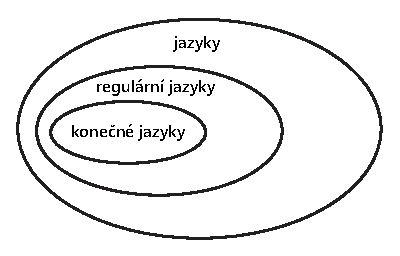
\includegraphics[width=8cm]{vajicko-1.eps}
\caption{Vychodilovo \uv{vajíčko.}}\label{obr-2}
\end{figure}

\begin{priklad}
\begin{eqnarray*}
N &=& \lbrace S \rbrace \\
\Sigma &=& \lbrace a, b \rbrace \\
P &=& \lbrace S \rightarrow aSb | \varepsilon \rbrace \\
L(G) = \lbrace a^{n}b^{n} | n \leq 0 \rbrace
\end{eqnarray*}
Máme tedy \emph{bezkontextový} jazyk.
\end{priklad}

\begin{priklad}
\begin{eqnarray*}
N &=& \lbrace S \rbrace \\
\Sigma &=& \lbrace a, b \rbrace \\
P &=& \lbrace S \rightarrow SS|aSb|bSa| \varepsilon \rbrace
\end{eqnarray*}
$L(G)$ je \emph{bezkontextový} jazyk.
\end{priklad}

\begin{priklad}
\begin{eqnarray*}
N &=& \lbrace S, V \rbrace \\
\Sigma &=& \lbrace p,),(, \Rightarrow, ! \rbrace \\
P &=& \lbrace S \rightarrow V|(S \Rightarrow S)|!S, V \Rightarrow pV|p \rbrace
\end{eqnarray*}
$L(G)$ je jazyk všech výrokových formulí.
\end{priklad}

\subsection{Gramatika nezkracující}
Gramatika G se nazývá nezkracující, pokud má pouze nezkracující pravidla a může mít pravidlo ve tvaru $S \rightarrow \varepsilon$, ale $S$ se nenechází na žádné z pravých stran.

\begin{priklad}
\begin{eqnarray*}
N &=& \lbrace S, A, B, C\rbrace \\
\Sigma &=& \lbrace a, b, c\rbrace \\
P &=& \lbrace S \rightarrow \varepsilon |abc|Ac, A \rightarrow aBcb, Bcb \rightarrow bBc, Bcc \rightarrow Ccc, bc \rightarrow Cb, aC \rightarrow aab|aA \rbrace
\end{eqnarray*}
\end{priklad}

\begin{veta}
Gramatiky typu 3 a 1 jsou nezkracující.
\end{veta}

\begin{veta}
Ke každé gramatice G, existuje ekvivalentní gramatika $G^{'}$, ve které jsou všechna pravidla obsahující terminální symboly ve tvaru $A \rightarrow a$, kde $A \in N, a \in \Sigma$.
\end{veta}

\begin{dukaz}
Pro každý termínál $a \in \Sigma$, zavedeme terminál $N_{a}$ a pravidlo $N_{a} \rightarrow a$.
Všechny výskyty terminálů ve výchozých pravidlech nahradíme přislušnými pomocnými neterminály.
$$
Bcb \rightarrow bBc \text{ se změní na } BN_{c}N_{b} \rightarrow N_{b} BN_{c}, 
N_{c} \rightarrow c, N_{b} \rightarrow b
$$
\end{dukaz}

\begin{veta}
Ke každé nekzracující gramatice existuje ekvivalentní gramatika, která je kontextově \mbox{závislá}.
\end{veta}

\begin{dukaz}
Předpokládejme, že $G = \langle N, \Sigma, P, S \rangle$ je nezkracující gramatika. Dle věty 7 můžeme předpokládat, 
že všechna pravidla jsou buď ve tvaru $A \rightarrow a$ (nevadí) nebo ve tvaru obecně. 
$A_{1} A_{2} \cdots A_{m} \rightarrow B_{1} B_{2} \cdots B_{n}$, kde $A_{1}, \ldots,A_{m}, B_{1}, \ldots,B_{n} \in N$ a navíc $m \leq n$. 
Tj. taková pravidla lze psát ve tvaru $A_{1} A_{2} \cdots A_{m} \rightarrow B_{1} B_{2} \cdots B_{my}$, kde $y = B_{m+1} \cdots B_{n}$ 
Budeme uvažovat nové pomocné neterminály $X_{1},...,X_{m}$ \footnote{pro každé pravidlo se uvažují zvlášť}. 
A zavedeme následující pravidla:
\begin{gather*}
A_{1} A_{2} \cdots A_{m} \rightarrow X_{1} A_{2} \cdots A_{m} \\
X_{1} A_{2} \cdots A_{m} \rightarrow X_{1} X_{2} A_{3} \cdots A_{m} \\
\vdots \\
X_{1} X_{2} \cdots X_{m-1} A_{m} \rightarrow X_{1} \cdots X_{m-1} X_{my} \\
X_{1} X_{2} \cdots X_{my} \rightarrow B_{1} X_{2} X_{3} \cdots X_{my} \\
\vdots \\
B_{1} B_{2} \cdots B_{m-1} X_{my} \rightarrow B_{1} B_{2} \cdots B_{m-1}B_{my}
\end{gather*}
Tento postup se aplikuje pro všechna pravidla. Hledaná gramatika $G^{'}$ se skládá z $\Sigma, N$ + všechny pomocné termínály + všechna odovozená pravidla.
\end{dukaz}

\subsection{Základní vlastnosti bezkontextových gramatik}
\begin{itemize}
\item
levá strana pravidla = jediný neterminál
\item
odvozování \uv{nezávisí na kontextu}
\end{itemize}

\begin{veta}
Mějme bezkontextovou gramatiku  $G = \langle N, \Sigma, P, S \rangle$ a nechť $X_{1} \cdots X_{k}, \ldots, z$ 
je P-derivace délky $n$, kde $X_{1}, \ldots, X_{k} \in (N \cup \Sigma)$ a $z \in (N \cup \Sigma)^{*}$ 
a potom pro každé $i = 1, \ldots, k$  existuje řetězec $z_{i} \in (N \cup \Sigma)^{*}$ 
a P-derivace $X_{i}, \ldots, z_{i}$ délky $n_{i}$ tak, že $z = z_{1} ,z_{2}, \ldots, z_{k}$ a $n = n_{1} + n_{2} + \cdots + n_{k}$
\end{veta}

\begin{dukaz}
Tvrzení prokázěmě induxí přes délku výchozí derivace $X_{1} \cdots X_{k}, \ldots, z$.
Pro $n = 0$: Triviální $z = X_{1} \cdots X_{k}, z_{i} = X_{i}, n_{i} = 0$. Každé $X_{i}$ je derivace délky 0. 
Nechť tvrzení platí pro libovolnou derivaci délky $n$ a dokážeme, že $X_{1} \cdots X_{k}$ je P-derivace délky $n + 1$.
Jelikož má uvažovaná P-derivace délku n + 1, lze ji psát ve tvaru:
$$
X_{1} \cdots X_{k}, \ldots, y \footnote{$X_{1} \cdots X_{k}, \ldots$, y má délku n}, z 
$$
Máme $y \Rightarrow_{G}z$. Můžeme aplikovat indukční předpoklad:
Existují řetězce $y_{1}, \ldots, y_{k}$ a P-derivace $X_{1}, \ldots, y_{1}$ až $X_{k}, \ldots, y_{k}$ 
délek $n_{1} \cdots n_{k}$ tak, že $y = y_{1} y_{2} \cdots y_{k}$ a $n = n_{1} + n_{2} + \cdots + n{k}$. 
Z faktu, že $y  \Rightarrow_{G}z$ a z toho, že gramatika je bezkontextová plyne, že $y$ je ve tvaru 
$y = y^{''} y^{'} A w^{'} w^{''}$ pro $i = 1, \ldots, k$. Pak $z$ je ve tvaru $z = y^{''} y^{'} u w^{'} w^{''}$ a $A \rightarrow n \in P$,
to jest $X_{i}, \ldots, y_{i}, y^{'} u w^{'}$ je P-derivce délky $n_{i+1}$. Hledáné derivace jsou:
\begin{gather*}
X_{1}, \ldots, y_{1} \\
\vdots \\
X_{i-1}, \ldots, y_{i-1} \\
X_{i}, \ldots, y_{i} y^{'} u w^{'} \\
X_{1+1}, \ldots, y_{i+1} \\
X_{k}, \ldots, j_{k} \\
\text{zkontrolovat!!}
\end{gather*}
\end{dukaz}

\begin{priklad}
\begin{eqnarray*}
N &=& \lbrace S \rbrace \\
\Sigma &=& \lbrace a, b \rbrace \\
P &=& \lbrace S \rightarrow SS|aS|bSa| \varepsilon \rbrace
\end{eqnarray*}
Posloupnost: $SbSaS, SbSa, SbaSba, aSbbaSba , abbaSba$ je P-derivace délky 4. \\*
Hledáme P-derivace:
\begin{enumerate}
\item
$S, aSb, ab$ (délka 2)
\item
$b$ (délka 0)
\item
$S, aSb$ (délka 1)
\item
$a$ (délka 0)
\item
$S, \varepsilon $ (délka 1)
\end{enumerate}
\end{priklad}

\begin{priklad}
Gramatika s jediným pravidlem $aBc \rightarrow abc$
\end{priklad}

\underline{Pozn.:} U regulárních a kontextových gramatik lze hned vidět, jestli $\varepsilon \in L(G)$.

Pro bezkontextovou gramatiku $G = \langle N, \Sigma, P,S \rangle$ zavedeme následující podmnožiny
\begin{gather*}
E_{0} = \lbrace A \in N | A \rightarrow \varepsilon \in P \rbrace \\
E_{i+1} = E_{i} \cup \lbrace A \in N | A \rightarrow x, \text{ kde } x \in E_{i}^* \rbrace
\end{gather*}

\begin{priklad}
\begin{eqnarray*}
A &\rightarrow& \varepsilon \\
B &\rightarrow& \varepsilon \\
E_{0} &=& \lbrace A, B \rbrace \\
E_{1} &=& \lbrace A, B, F \rbrace \\
E_{2} &=& \lbrace A, B, F, G \rbrace
\end{eqnarray*}
$$
E_{i} \subseteq N, E_{N} = \bigcup_{i=0}^{\infty} E_{i}
$$
Jelikož je $N$ konečná, musí platit:
\begin{gather*}
E_{0} \subseteq E_{1} \subseteq E_{2} \subseteq \cdots \subseteq E_{i} = E_{i+1} = E_{i+2} \\
E_{N} = E_{i}
\end{gather*}
\end{priklad}

\begin{veta}
Pro každou bezkontextovou gramatiku $G = \langle N, \Sigma, P,S \rangle$ a pro příslušné $E_{N}$ platí nasledující $A \Rightarrow_{G}^{*}\varepsilon$, pak $A \in E_{N}$. 
Speciálně $\varepsilon \in L(G)$, pak $S \in E_{N}$.
\end{veta}

\begin{dukaz}
Prokážeme obě implikace: \\
Pokud $A \Rightarrow_{G}^{*}\varepsilon$, pak prokážeme indukci přes délku P-derivace, tj. triviální případ je $A \Rightarrow_{G}\varepsilon$, 
tj. existuje pravidlo $A \rightarrow \varepsilon \in P$ tj. $A \in E_{0}$.
Předpokládejme, že tvrzení platí pro všechny P-derivace délky $n$.
Mějme $A, \ldots, \varepsilon$ P-derivace délky n + 1. Použitím předchozí věty $(A, X_{1} \cdots X_{k}, \ldots, \varepsilon)$ $A, X_{i} \cdots X_{n}, \ldots, \varepsilon$.
Tzn. existují derivace $X_{i}, \ldots, \varepsilon$ délek nejvýše $n$. Z předpokladu $X_{i} \in E_{n}$, pro každé $i$ tj. i $A \in E_{N}$. 
$\Leftarrow$ Dokáže, že pro každé $E_{i}$ platí, pokud $E \in E_{i}$ pak $A \Rightarrow_{G}^{*}\varepsilon$. Pro $E_{0}$ zřejmé.
$A \rightarrow X_{0} \cdots X_{k}, A \in E_{j}$.
\end{dukaz}

\begin{veta}
Pro každou bezkontextovou gramatiku $G$, existuje bezkontextová gramatika $G^{'}$ neobsahující $\varepsilon$ pravidla tak, že $L(G) \setminus \lbrace \varepsilon \rbrace = L(G^{'})$.
\end{veta}

\begin{dukaz}
$\ldots$
\end{dukaz}

%\newpage
\renewcommand{\indexcolumns}{3}
\printindex
\end{document}